\documentclass[12pt]{article}

\usepackage{sbc-template}
\usepackage{graphicx,url}
\usepackage[utf8]{inputenc}
\usepackage[brazil]{babel}
\usepackage[latin1]{inputenc} 
\usepackage{amsmath}

\sloppy

\title{Desenvolvimento de uma Arquitetura de IoT para Medições e
Monitoramento de Resíduos Sólidos}

%\author{Felipe J. dos S.\inst{1}, Stephanie K. A. De Sousa\inst{2}, Rubens D. S. Matos Jr.\inst{3} Fabio L. Sá P.\inst{4}}


%\address{Instituto Federal de Educação, Ciência e Tecnologia de Sergipe
%  (IFS)\\
%  Lagarto -- SE -- Brazil
%}

\begin{document}

\maketitle

\begin{abstract}
This article addresses the use of emerging technologies in urban solid waste management, with emphasis on the Internet of Things (IoT) and the MQTT communication protocol. We explore the significant contributions of these technologies, as well as the challenges associated with their implementation in real-world scenarios. The strategic choice of the MQTT protocol proved crucial for the development of robust and efficient waste measurement and monitoring systems. Through systematic literature reviews, project analysis, and practical implementation, we identify a range of practical applications of emerging technologies in solid waste management. Case studies and practical examples highlight how IoT-based systems can optimize collection routes, reduce costs, and improve waste management efficiency. However, we acknowledge the challenges faced in adopting these technologies, including dependence on advanced infrastructure, data security issues, and public acceptance. This study contributes to the understanding and practical application of emerging technologies in urban solid waste management, providing a solid foundation for future research and improvements in the quest for more sustainable and efficient solutions.
\end{abstract}
     
\begin{resumo} 
Este artigo aborda o uso de tecnologias emergentes na gestão de resíduos sólidos urbanos, com ênfase na Internet das Coisas (IoT) e no protocolo de comunicação MQTT. Exploramos as contribuições significativas dessas tecnologias, bem como os desafios associados à sua implementação em cenários reais. A escolha estratégica do protocolo MQTT revelou-se crucial para o desenvolvimento de sistemas robustos e eficientes de medição e monitoramento de resíduos. Por meio de revisões sistemáticas da literatura, análise de projetos e implementação prática, identificamos uma série de aplicações práticas das tecnologias emergentes na gestão de resíduos sólidos. Estudos de caso e exemplos práticos destacaram como sistemas baseados em IoT podem otimizar rotas de coleta, reduzir custos e melhorar a eficiência na gestão de resíduos. No entanto, reconhecemos os desafios enfrentados na adoção dessas tecnologias, incluindo a dependência de infraestrutura avançada, questões de segurança de dados e aceitação pública. Este estudo contribui para a compreensão e aplicação prática das tecnologias emergentes na gestão de resíduos sólidos urbanos, fornecendo uma base sólida para pesquisas futuras e aprimoramentos na busca por soluções mais sustentáveis e eficientes.
\end{resumo}

\section{Introdução}

A gestão eficiente dos resíduos sólidos urbanos é um desafio crescente enfrentado pelas cidades em todo o mundo. Com o aumento da população e o desenvolvimento urbano contínuo, torna-se imperativo adotar abordagens inovadoras para lidar com essa problemática de forma sustentável. Como destacado por \cite{anagnostopoulos2017challenges}, a gestão de resíduos sólidos em ambientes urbanos apresenta desafios complexos que exigem soluções abrangentes e adaptáveis.

Nesse contexto, as tecnologias emergentes, como a Internet das Coisas (IoT), desempenham um papel crucial na transformação da gestão de resíduos sólidos. Segundo \cite{Bouskela2016TheRT}, a transição de modelos tradicionais de gerenciamento para abordagens mais inteligentes e conectadas é essencial para enfrentar os desafios contemporâneos relacionados aos resíduos urbanos.

Este artigo busca explorar e desenvolver soluções inovadoras para a gestão de resíduos sólidos urbanos, integrando tecnologias como IoT e o protocolo de comunicação MQTT. Através de uma revisão da literatura, análise de projetos e implementação prática, pretendemos identificar contribuições significativas e desafios associados ao uso dessas tecnologias em cenários reais.

Ao longo deste artigo, serão apresentados estudos de caso, exemplos práticos e reflexões sobre as oportunidades e desafios na aplicação das tecnologias emergentes na gestão de resíduos sólidos. Espera-se que este trabalho contribua para uma compreensão mais ampla das possibilidades oferecidas pela IoT e outras tecnologias na busca por soluções mais eficientes e sustentáveis para a gestão de resíduos sólidos urbanos.

\section{Desafios na Gestão de Resíduos Sólidos} \label{sec:Desafios na Gestão de Resíduos Sólidos}

A gestão eficaz de resíduos sólidos urbanos enfrenta uma série de desafios complexos que demandam abordagens inovadoras e adaptáveis. O aumento populacional e o crescimento das áreas urbanas têm gerado uma quantidade cada vez maior de resíduos, ampliando a pressão sobre os sistemas de gerenciamento existentes \cite{hoornweg2012waste}. Essa crescente demanda por serviços de coleta, transporte e disposição de resíduos implica em desafios logísticos significativos, especialmente em áreas densamente povoadas, onde a infraestrutura muitas vezes não acompanha o ritmo do crescimento urbano.

Além disso, a má gestão dos resíduos sólidos contribui para uma série de problemas ambientais e de saúde pública. A falta de conscientização sobre a separação adequada dos resíduos, aliada à ineficácia dos sistemas de coleta e disposição, resulta em práticas inadequadas de descarte que podem contaminar o solo, a água e o ar \cite{OPAS}. A poluição gerada pelos resíduos, além de representar uma ameaça à biodiversidade, também compromete a qualidade de vida das comunidades urbanas.

Um dos desafios-chave enfrentados na gestão de resíduos sólidos é a necessidade de monitoramento e controle ao longo de toda a cadeia de gestão. \cite{HANNAN20112406} destacam a importância do rastreamento e identificação eficazes dos resíduos, desde sua geração até sua disposição final, para garantir uma gestão adequada e responsável. No entanto, sistemas tradicionais de monitoramento muitas vezes carecem de precisão e eficiência, dificultando a tomada de decisões informadas e a implementação de medidas corretivas.

Além dos desafios operacionais, a gestão de resíduos sólidos enfrenta pressões crescentes relacionadas à sustentabilidade e mitigação das mudanças climáticas. Conforme destacado pelo \cite{IPCC_2023}, a gestão inadequada de resíduos pode resultar em emissões significativas de gases de efeito estufa, contribuindo para o aquecimento global e outros impactos ambientais adversos. Portanto, a busca por soluções que reduzam o impacto ambiental dos resíduos e promovam a economia circular torna-se uma prioridade urgente.

Diante desses desafios, torna-se evidente a necessidade de abordagens inovadoras e integradas na gestão de resíduos sólidos urbanos. A utilização de tecnologias emergentes, como a Internet das Coisas (IoT), oferece oportunidades promissoras para superar esses desafios, permitindo uma gestão mais eficiente, sustentável e responsável dos resíduos urbanos.

'\section{Metodologia}

Nesta seção, descrito a metodologia para implementação do sistema de medição e monitoramento, incluindo e os componentes eletrônicos essenciais desenvolvido para controle e aquisição de dados. A arquitetura do projeto é organizada em três camadas: dispositivos físicos, infraestrutura de comunicação e interface, otimizando a funcionalidade e escalabilidade do sistema.

\begin{figure}[h]
  \centering
  \caption{Arquitetura de 3 camadas.}
  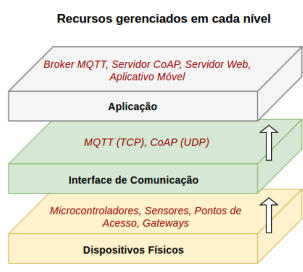
\includegraphics[width=0.4\textwidth]{Figuras/camadas.png}
  \vspace{-5pt} % Ajuste o espaçamento conforme necessário
  \begin{center}
    \small Fonte: \cite{de2018arquitetura}
  \end{center} 
\end{figure}

Na camada de dispositivos físicos, foi adotado o ESP32~\cite{esp32-datasheet}, o sensor ultrassônico HC-SR04~\cite{hcsr04-datasheet} e o sensor DHT11~\cite{dht11-datasheet}, cada um desempenhando um papel específico no processo de medição e monitoramento.

O ESP32 foi escolhido como a plataforma principal devido à sua versatilidade e à presença integrada de um módulo Wi-Fi, possibilitando a conectividade sem fio para a transmissão eficiente de dados para a nuvem na segunda camada do sistema. O módulo Wi-Fi incorporado no ESP32 oferece uma solução conveniente e econômica para a comunicação remota, tornando-o uma escolha ideal para projetos que exigem conectividade online. Além disso, o sensor ultrassônico HC-SR04 é empregado para medir a distância entre o sensor e objetos nas proximidades, sendo crucial para o monitoramento do nível de enchimento da lixeira de forma precisa e eficiente em tempo real. Já o sensor DHT11 é utilizado para monitorar a temperatura e a umidade no ambiente circundante da lixeira, fornecendo informações valiosas sobre as condições ambientais que podem influenciar o nível de enchimento da mesma.

Na camada de comunicação, adotamos o protocolo MQTT (Message Queuing Telemetry Transport) para viabilizar a comunicação eficiente e assíncrona entre os dispositivos físicos e a nuvem. O MQTT é reconhecido por sua eficácia e simplicidade, sendo amplamente utilizado em aplicações de IoT.

Uma das principais vantagens do MQTT em projetos de IoT é sua capacidade de lidar com redes instáveis e dispositivos com restrições de energia, minimizando a sobrecarga de comunicação e garantindo eficiência energética. Além disso, o MQTT oferece escalabilidade, possibilitando a conexão e comunicação eficiente entre um grande número de dispositivos distribuídos. Sua estrutura leve e a capacidade de garantir a entrega de mensagens, mesmo em condições de rede intermitente, fazem dele uma escolha preferencial para implementações IoT.

O MQTT opera sob o paradigma de publicação/assinatura (\textit{publish/subscribe}), oferecendo uma abordagem flexível para a comunicação entre dispositivos, com os papéis principais de \textit{publisher} (publicador) e \textit{subscriber} (assinante).

O broker MQTT atua como intermediário na comunicação entre dispositivos, recebendo mensagens dos publicadores e encaminhando-as aos assinantes. No projeto, escolhemos o \textit{HiveMQ} devido à sua gratuidade e facilidade de uso, desempenhando um papel crucial na troca de dados entre os ESP32 e a nuvem. Os tópicos no MQTT funcionam como canais virtuais para enviar ou receber mensagens, organizando a comunicação. Cada mensagem é associada a um tópico específico, como temperatura, umidade e nível de enchimento da lixeira neste projeto, garantindo direcionamento preciso das informações. As ações de \textit{subscribe} e \textit{publish} permitem uma comunicação bidirecional eficiente entre os dispositivos.

A adoção do MQTT na camada de comunicação proporciona uma arquitetura distribuída e eficiente. Os ESP32, como publicadores MQTT, enviam dados aos tópicos relevantes, enquanto o \textit{HiveMQ} gerencia a comunicação entre dispositivos e a nuvem. O diagrama apresentado na Figura 2 ilustra essa arquitetura.

\begin{figure}[h]
  \centering
  \caption{Diagrama de Sequência das ações de publish/subscriber da aplicação}
  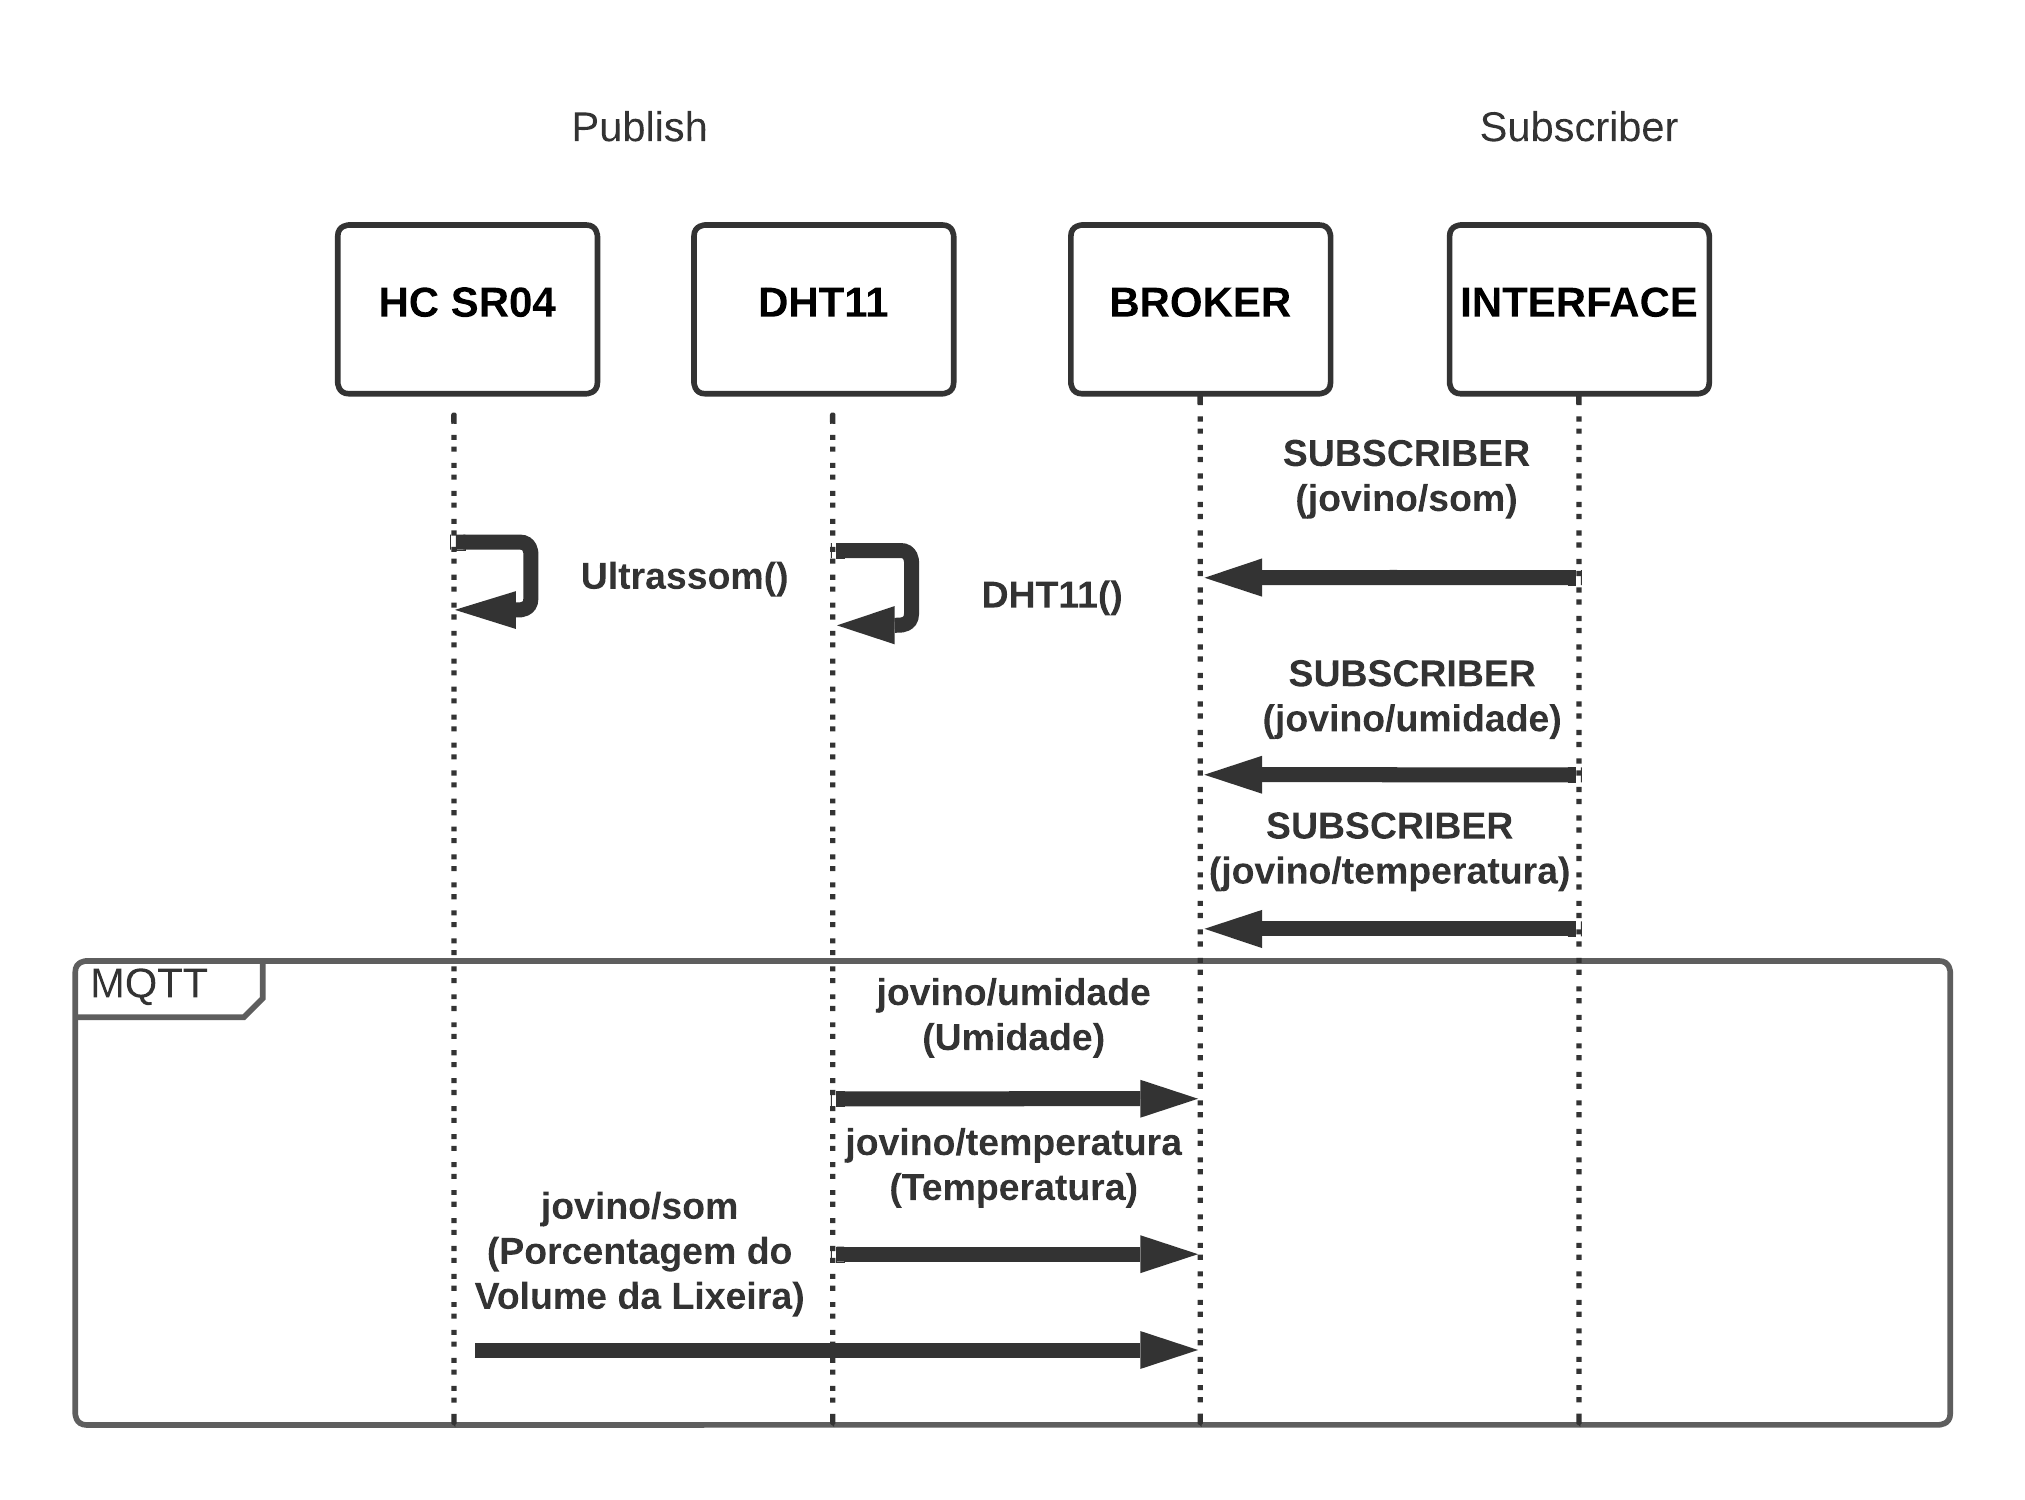
\includegraphics[width=0.8\textwidth]{Figuras/mqtt.png}
  \vspace{-5pt} % Ajuste o espaçamento conforme necessário
  \begin{center}
    \small Fonte: Autor
  \end{center}
\end{figure}

Na terceira camada do sistema, a interface de usuário proporciona uma maneira intuitiva de visualizar e interagir com os dados provenientes dos dispositivos físicos. Utilizamos o aplicativo de celular \textit{MQTT Dashboard} devido à sua conveniência, variedade de soluções de exibição MQTT e facilidade de uso em dispositivos móveis.

O \textit{MQTT Dashboard} atua como uma interface gráfica para exibir dados recebidos via MQTT. Ele permite a criação de \textit{widgets} personalizados para representar informações específicas, como gráficos, medidores e contadores, além de oferecer interação com os dispositivos para controle remoto de funcionalidades.

A escolha do \textit{MQTT Dashboard} baseou-se em sua simplicidade e facilidade de uso, além da disponibilidade gratuita, tornando-o uma opção prática para monitoramento e controle remoto do sistema por meio de dispositivos móveis.

Essa camada completa a arquitetura de 3 camadas do sistema, fornecendo uma plataforma eficiente para visualização e interação com os dados provenientes dos ESP32, e oferecendo uma solução abrangente para o monitoramento remoto de lixeiras, com uma interface intuitiva acessível através do \textit{MQTT Dashboard}.

Para instaurar o sistema de medição e monitoramento de resíduos sólidos, empregou-se o cálculo da porcentagem do volume por meio de um sensor ultrassônico. Esta medida é relativa e expressa pela seguinte fórmula:

\[
\text{percentMax} = \left( \frac{\text{distancia}}{\text{Tmax}} \right) \times 100
\]

Para calcular a porcentagem do volume desejada (\(\text{percentMax}\)), é necessário considerar a distância medida pelo sensor ultrassônico (\(\text{distancia}\)) em relação ao valor máximo permitido (\(\text{Tmax}\)). Este cálculo fornece uma representação da distância medida em relação ao valor máximo permitido.

\subsection{Testes}

Nesta seção, apresentamos uma síntese dos testes conduzidos para validar o funcionamento do sistema de medição e monitoramento em diferentes cenários, garantindo sua robustez e confiabilidade.

Para verificar a recepção de informações via MQTT, conduzimos testes com um sensor ultrassônico HC-SR04, um ESP32, uma régua e a infraestrutura MQTT configurada. Confirmamos a comunicação efetiva entre o sensor e o servidor MQTT, validando o envio de informações correspondentes. Durante os testes, foi observada a leitura precisa das informações do sensor em relação a um obstáculo posicionado na régua, com sucesso na transmissão desses dados para o servidor MQTT. O objetivo era validar o funcionamento do MQTT e do aplicativo de exibição.

Além disso, realizamos um teste para avaliar o envio de informações, utilizando um LED, um resistor de 220 ohms, um ESP32 e a comunicação MQTT. Verificamos a capacidade do sistema de controlar dispositivos remotos, confirmando o acionamento correto do LED através do ESP32 durante o teste.

A capacidade do sistema em lidar com múltiplos dispositivos simultaneamente foi testada através de um experimento com dois ESP32, cada um representando uma lixeira. Não houve conexão direta entre os dispositivos. Utilizamos sensores ultrassônicos HC-SR04 para medir a distância entre os sensores e os objetos próximos às lixeiras. Durante o teste, implementamos uma estratégia eficiente de coleta de dados simultânea, garantindo a transmissão eficaz dessas informações para o servidor MQTT. Cada lixeira foi associada a tópicos específicos para uma organização clara e sem mistura de dados.

Para testar o sensor DHT11, montamos um ambiente experimental com um ESP32, um sensor DHT11, um soprador térmico e um borrifador de água. O ESP32 foi programado para ler os dados do sensor DHT11 e transmiti-los através do protocolo MQTT para um servidor MQTT. O soprador térmico foi utilizado para simular variações de temperatura no ambiente de teste, enquanto o borrifador de água introduziu alterações na umidade relativa. Os resultados indicaram o funcionamento do sensor DHT11 em relação às variações de temperatura e umidade, com leituras consistentes que refletiram adequadamente as mudanças nas condições do ambiente experimental.

\begin{figure}[h]
  \centering
  \caption{Interface do MQTT Dashboard}
  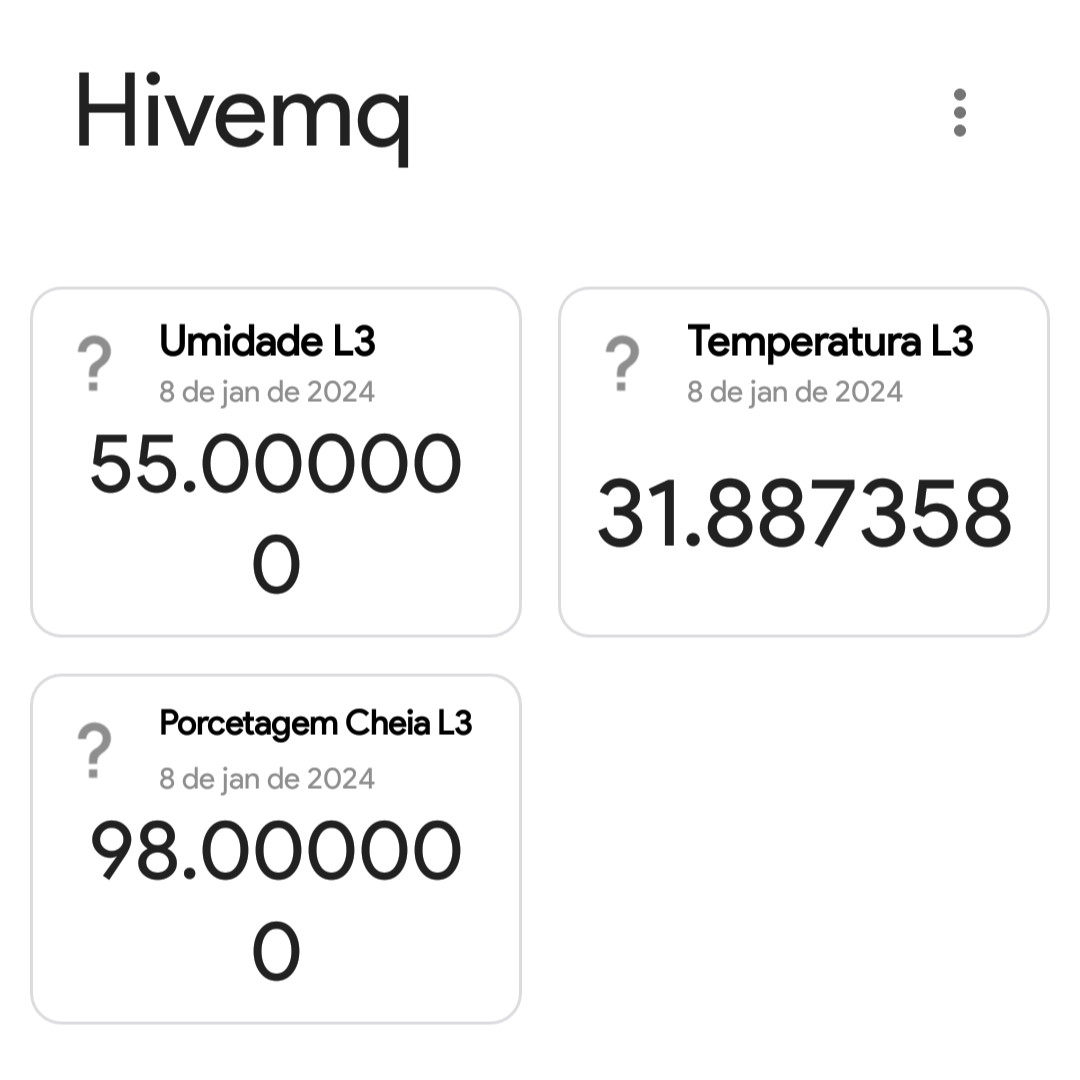
\includegraphics[width=0.3\textwidth]{Figuras/dashboard.jpg}
  \vspace{-10pt} % Ajuste o espaçamento conforme necessário
  \begin{center}
    \small Fonte: Autor
  \end{center}
\end{figure}

\section{Estudos de Caso e Exemplos Práticos}

\cite{2010Sruthi} O trabalho publicado pelos autores Sruthi K V e Manjunath K N foi um sistema de medição que integra sensores ultrassônicos, resistores de sensibilidade à pressão, visando estabelecer um eficiente sistema de coleta de resíduos. Centralizado em torno do controlador ARM LPC2148, um dispositivo de 32 bits, o sistema utiliza o sensor ultrassônico HC-SR04 para avaliação dos níveis de lixo e o sensor de resistência à pressão para medição do peso. A comunicação foi assegurada pelo GSM SIM900 para envio de mensagens ao administrador, enquanto o RFID desempenhou o papel de autenticação dos usuários. A interface HTML foi empregada para fornecer um \textit{site} acessível a todos, permitindo a visualização dos contentores de lixo cheios. Destaca-se tambfoim a utilização do SQL como banco de dados para armazenamento eficiente dos dados provenientes dos sensores, proporcionando uma gestão robusta e integrada do sistema de coleta de resíduos. Essa abordagem, proposta no trabalho, representa um avanço significativo na otimização dos processos de coleta de resíduos, demonstrando a sinergia entre tecnologias diversas para a eficiência e sustentabilidade do sistema.

\cite{HANNAN20112406} O trabalho se fundamenta na análise do sistema de monitoramento inteligente de lixeiras e caminhões, destacando-se pela integração estratégica de diversas tecnologias. Entre elas, destacam-se RFID, GPS, GPRS, GIS e câmeras, com o objetivo de coletar dados em tempo real e fornecer informações cruciais para a gestão eficiente de resíduos sólidos.

O sistema utiliza \textit{tags} RFID para identificação e rastreamento das lixeiras, fornecendo informações como o ID e a data da coleta. O rastreamento em tempo real é viabilizado por módulos GPS nos caminhões, garantindo alta precisão na localização. A transmissão remota dos dados coletados, incluindo informações RFID, dados GPS e imagens das lixeiras, é assegurada pelos módulos GPRS.

A aplicação da tecnologia GIS possibilita a visualização e mapeamento das informações, enquanto câmeras de baixo custo capturam imagens das lixeiras para análise do seu status. Um banco de dados é incorporado ao sistema para armazenamento e compilação das informações, viabilizando o monitoramento e a gestão eficaz das atividades de coleta de resíduos sólidos.

A convergência dessas tecnologias permite a coleta de dados em tempo real, análise eficiente e tomada de decisões informadas, proporcionando uma abordagem abrangente para aprimorar a gestão de resíduos sólidos no contexto contemporâneo. A abordagem apresentada reflete avanços significativos na aplicação prática e integrada de tecnologias para otimizar a eficiência e sustentabilidade dos sistemas de gerenciamento de resíduos sólidos.

\cite{de2018arquitetura} O trabalho apresentou uma arquitetura baseada em Internet das Coisas (IoT) para o monitoramento e medição do nível de resíduos em lixeiras públicas. Os pontos positivos do trabalho incluíram a proposta de uma solução inovadora que utilizava tecnologias modernas para melhorar a gestão de resíduos, a possibilidade de monitoramento remoto em tempo real e a sugestão de utilização de algoritmos de Inteligência Artificial para análise de dados históricos e previsões futuras relacionadas à quantidade de resíduos descartados e à frequência da coleta.

No entanto, a complexidade da implementação da arquitetura proposta foi considerada um ponto negativo, conforme mencionado no trabalho. Além disso, foi importante considerar que a implementação de tecnologias IoT poderia exigir investimentos significativos em infraestrutura e treinamento de pessoal, representando um desafio para algumas organizações.

Em resumo, o trabalho ofereceu uma abordagem inovadora para a gestão de resíduos, com ênfase na utilização de tecnologias IoT e análise de dados para melhorar a eficiência da coleta de resíduos. No entanto, foi importante considerar os desafios e custos associados à implementação de uma solução baseada em IoT.

\section{Conclusão}

O presente estudo explorou as potenciais aplicações das tecnologias emergentes na gestão de resíduos sólidos urbanos, com foco na Internet das Coisas (IoT) e no protocolo de comunicação MQTT. Ao longo da pesquisa, investigamos as contribuições significativas dessas tecnologias, bem como os desafios associados à sua implementação em cenários reais.

A escolha estratégica do protocolo MQTT demonstrou ser fundamental para o desenvolvimento de sistemas robustos e eficientes de medição e monitoramento de resíduos. Sua capacidade de lidar com redes instáveis e dispositivos com restrições de energia proporcionou uma base sólida para a construção de sistemas resilientes, essenciais na gestão moderna de resíduos.

Através de revisões sistemáticas da literatura, análise de projetos e implementação prática, identificou-se uma série de aplicações práticas das tecnologias emergentes na gestão de resíduos sólidos. Estudos de caso e exemplos práticos demonstraram como sistemas baseados em IoT podem otimizar rotas de coleta, reduzir custos e melhorar a eficiência na gestão de resíduos.

No entanto, também reconhecemos os desafios enfrentados na adoção dessas tecnologias, incluindo a dependência de infraestrutura avançada, questões de segurança de dados e aceitação pública. Esses desafios destacam a necessidade de abordagens multidisciplinares e estratégias de adoção progressiva na implementação de tecnologias emergentes na gestão de resíduos.

Em resumo, este estudo contribui para a compreensão e aplicação prática das tecnologias emergentes na gestão de resíduos sólidos urbanos. A metodologia desenvolvida proporcionou uma base sólida para a realização deste estudo, bem como para pesquisas futuras e aprimoramentos práticos na busca por soluções mais sustentáveis e eficientes na gestão de resíduos sólidos urbanos.

\bibliographystyle{sbc}
\bibliography{sbc-template}

\end{document}
